%\documentclass[border=5mm,varwidth]{standalone}
\documentclass[border=5mm]{standalone}
\usepackage{tikz}
\newcommand\spiral{}% Just for safety so \def won't overwrite something
\def\spiral[#1](#2)(#3:#4:#5){% \spiral[draw options](placement)(end angle:revolutions:final radius)
\pgfmathsetmacro{\domain}{pi*#3/180+#4*2*pi}
\draw [#1,shift={(#2)}, domain=0:\domain,variable=\t,smooth,samples=int(\domain/0.08)] plot ({\t r}: {#5*\t/\domain})
}

\begin{document}
\begin{tikzpicture}
    \draw [->, domain=0:20,variable=\t,smooth,samples=75]
    plot ({\t r}: {0.02*\t*\t});
\end{tikzpicture}

\begin{tikzpicture}
    \spiral[red](0,0)(0:6:6);
    \spiral[blue](0,0)(0:6:-6);
    \spiral[blue](-12,0)(0:6:6);
    \spiral[red](12,0)(0:6:-6);
    \spiral[blue](-12,0)(90:2:-2.25);
    \spiral[red](12,0)(90:2:2.25);
\end{tikzpicture}

\newline
\centering
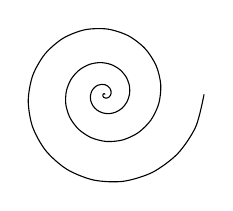
\begin{tikzpicture}
    \draw [domain=0:25.1327,variable=\t,smooth,samples=75]
    plot ({\t r}: {0.002*\t*\t});
\end{tikzpicture}

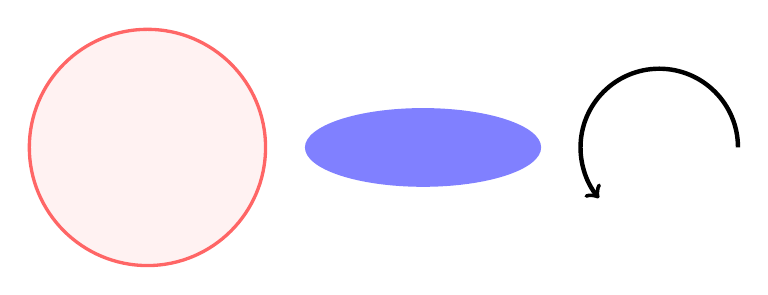
\begin{tikzpicture}
\filldraw[color=red!60, fill=red!5, very thick](-1,0) circle (1.5);
\fill[blue!50] (2.5,0) ellipse (1.5 and 0.5);
\draw[ultra thick, ->] (6.5,0) arc (0:220:1);
\end{tikzpicture}

\end{document}
